\documentclass{report}
\usepackage{pdfpages}
\usepackage[a4paper, top=2cm, bottom=2cm, left=2cm, right=2cm]{geometry}
\usepackage{fancyhdr}
\usepackage{amsmath} % Für mathematische Symbole
\usepackage{amssymb} % Für \mathbb
\usepackage[linesnumbered,ruled]{algorithm2e} % Für Algorithmus-Umgebung
\usepackage{ulem}
\usepackage{xcolor}
\usepackage{array}
\usepackage{graphicx}
\usepackage{listings}
\usepackage{xcolor}
\usepackage{naive-ebnf}
\usepackage[utf8]{inputenc}
\usepackage[absolute,overlay]{textpos}
\usepackage{tcolorbox}

\lstdefinestyle{cppstyle}{
    language=C++,             % Specify the language
    basicstyle=\ttfamily,     % Set the font to typewriter
    basicstyle=\ttfamily\footnotesize,
    keywordstyle=\color{blue}\bfseries, % Keywords in bold blue
    commentstyle=\color{green},         % Comments in green
    stringstyle=\color{red},            % Strings in red
    numbers=left,            % Line numbers on the left
    numberstyle=\tiny\color{gray}, % Line numbers in tiny gray font
    stepnumber=1,             % Line number step
    breaklines=true,          % Automatic line breaking
    tabsize=4,                % Set tab size
    showstringspaces=false,   % Don't show spaces in strings
    frame=single,             % Add a frame around the code
}

\newcommand{\name}{Marco Söllinger}
\newcommand{\fach}{SEN2}
\newcommand{\topic}{Übung 1}
\newcommand{\uebungangabe}{Uebung1.pdf}

\newcommand{\matnr}{s2410306011}
\newcommand{\uebungsgruppe}{Gruppe 1}
\newcommand{\aufwand}{2}


\pagestyle{fancy}
\normalem 
\fancyhead[R]{Marco Söllinger}  

\begin{document}
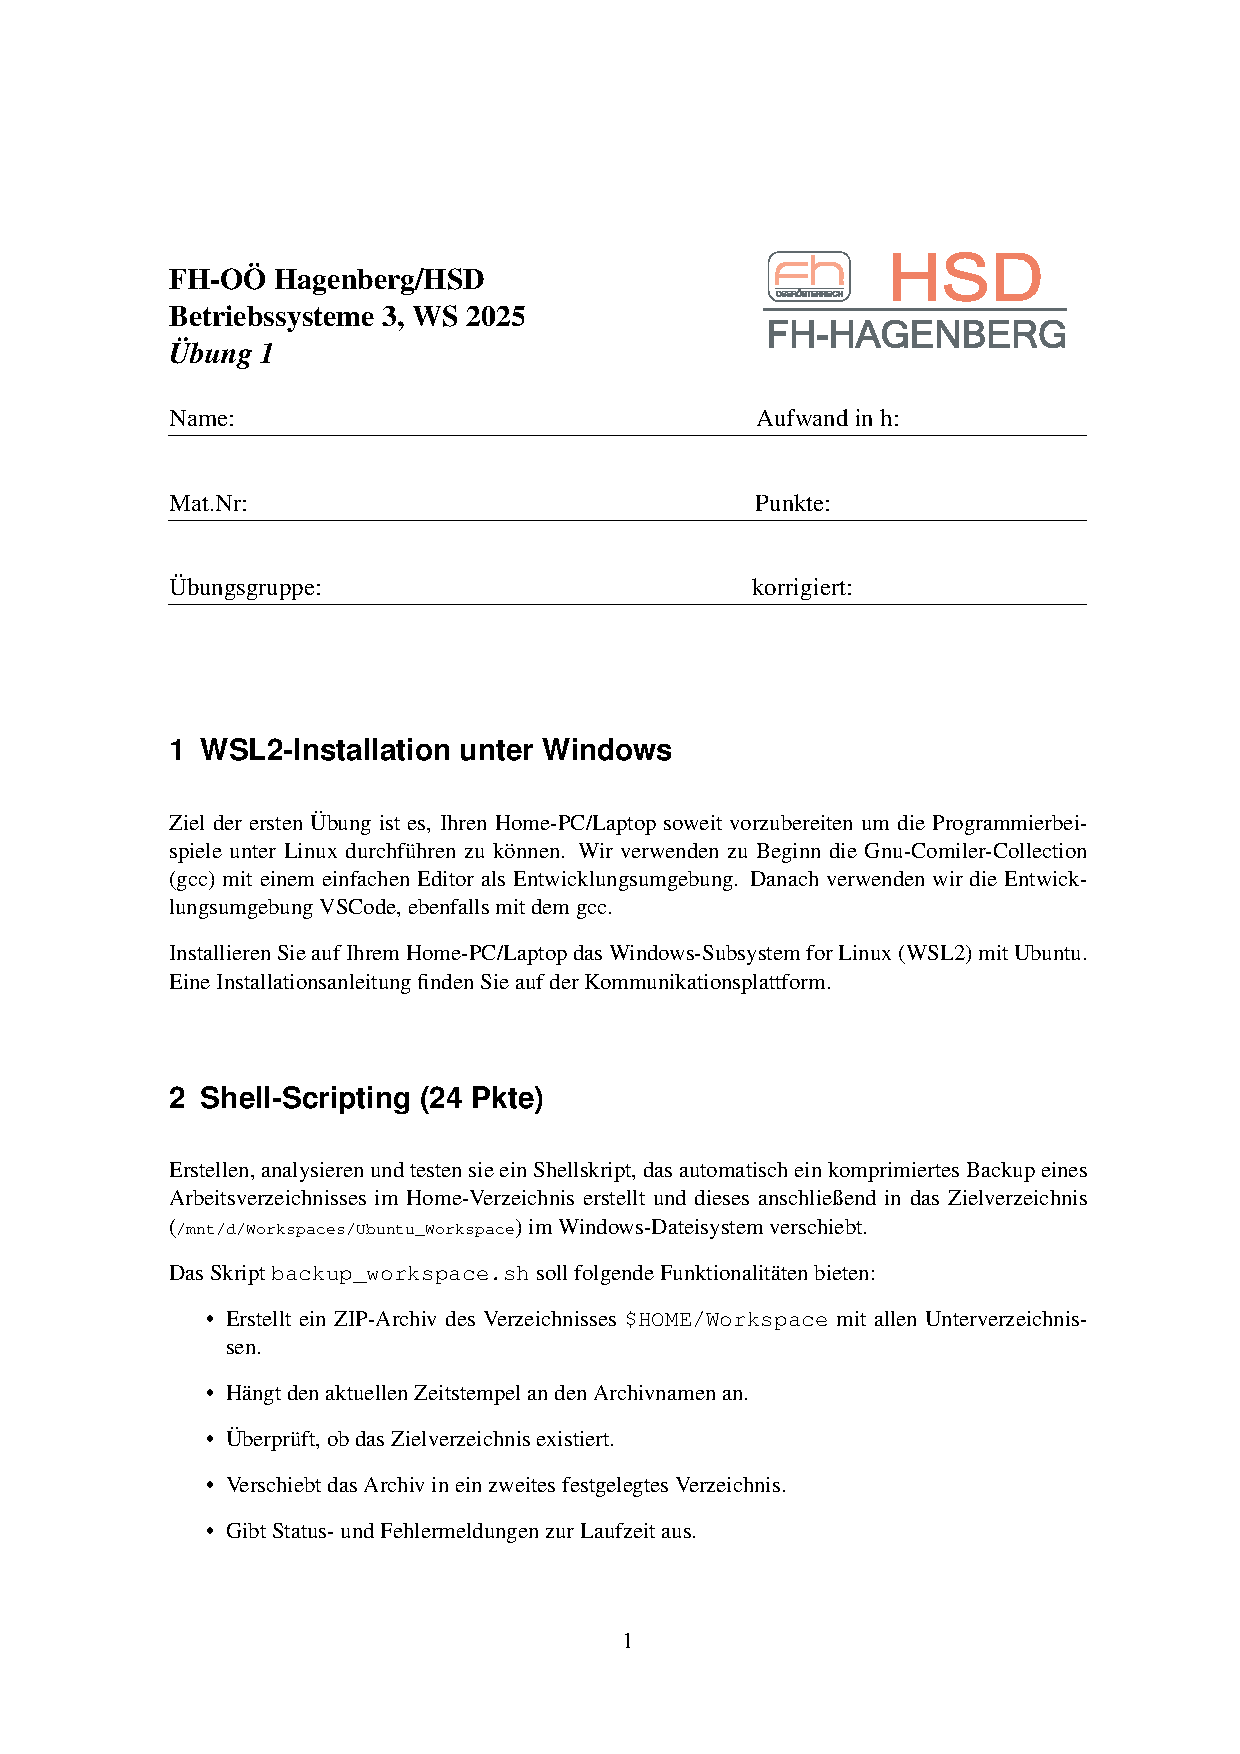
\includepdf[pages=1,pagecommand={
			\begin{textblock*}{5cm}(5.5cm, 6.9cm)
				\textbf{\name}
			\end{textblock*}
			\begin{textblock*}{5cm}(5.5cm, 8.4cm)
				\textbf{\matnr}
			\end{textblock*}
			\begin{textblock*}{5cm}(5.5cm, 9.8cm)
				\textbf{\uebungsgruppe}
			\end{textblock*}
			\begin{textblock*}{5cm}(15.3cm, 6.9cm)
				\textbf{\aufwand}
			\end{textblock*}
		}]{Uebung1-1.pdf}
\includepdf[pages=2-]{Uebung1-1.pdf}

\section*{Beispiel 1}
In dieser Aufgabe wurde das backup\_workspace Skript erstellt, welches den aktuellen Stand des Arbeitsverzeichnisses sichert.\\
Der Aufruf erfolgt über die Kommandozeile mit dem Befehl:\\
\begin{lstlisting}[style=cppstyle, title=\texttt{Terminal Output}]
./backup_workspace.sh <tmp location> <Backup Name> [-i input_directory] [-o output_directory]
  -i    Specify the input directory (default: /home/flashfish/Workspace)
  -o    Specify the output directory (default: /home/flashfish/Backups)
\end{lstlisting}
"tmp location" und "Backup Name" sind Pflichtangaben, wie in der Angabe beschreiben.\\
Falls "tmp location" nicht existiert, wird dieser erstellt.\\
Bei "backup name" wird zusaetzlich noch das aktuelle Datum und Uhrzeit angehaengt.\\\\
-i und -o sind optionale Parameter, welche das Eingabe- und Ausgabe-Verzeichnis angeben.\\
Als Standardwerte werden \$HOME/Workspace und \$HOME/Backups verwendet, wobei das Input-Verzeichnis existieren muss und das Output-Verzeichnis erstellt wird, falls es nicht existiert.\\\\\\
Bei dem Skript wird zuerst überprüft, ob die Pflichtangaben übergeben wurden, und ob die Parameter der Verzeichnisse gültig sind.\\


\subsection*{3.2 Code}
\lstinputlisting[style=cppstyle, title=\texttt{backup\_workspace} ]{../backup_workspace.sh}

\subsection*{3.3 Test}

Test 1: Kein Argument übergeben
\begin{lstlisting}[style=cppstyle, title=\texttt{Terminal Output}]
flashfish@fedora-4 ~/D/R/F/B/Uebung01 (main) [1]> ./backup_workspace.sh
Error: Not enough arguments provided.
Usage: ./backup_workspace.sh <tmp location> <Backup Name> [-i input_directory] [-o output_directory]
  -i    Specify the input directory (default: /home/flashfish/Workspace)
  -o    Specify the output directory (default: /home/flashfish/Backups)
\end{lstlisting}
Test 2: Nur tmp location übergeben
\begin{lstlisting}[style=cppstyle, title=\texttt{Terminal Output}]
flashfish@fedora-4 ~/D/R/F/B/Uebung01 (main) [1]> ./backup_workspace.sh
Error: Not enough arguments provided.
Usage: ./backup_workspace.sh <tmp location> <Backup Name> [-i input_directory] [-o output_directory]
  -i    Specify the input directory (default: /home/flashfish/Workspace)
  -o    Specify the output directory (default: /home/flashfish/Backups)
\end{lstlisting}
Test 3: Output-Verzeichnis und temp location sind gleich
\begin{lstlisting}[style=cppstyle, title=\texttt{Terminal Output}]
flashfish@fedora-4 ~/D/R/F/B/Uebung01 (main)> ./backup_workspace.sh ~/Backups test
  adding: Workspace/ (stored 0%)
  adding: Workspace/Testfolder1/ (stored 0%)
  adding: Workspace/Testfolder1/Test1.txt (stored 0%)
  adding: Workspace/Testfolder1/test2.txt (stored 0%)
  adding: Workspace/Testfolder2/ (stored 0%)
  adding: Workspace/Testfolder2/o.txt (stored 0%)
ZIP created successfully
Backup process completed successfully.
\end{lstlisting}
Test 4: Aufruf mit Temp location innerhalb Input-Verzeichnis (Hat funktioniert)
\begin{lstlisting}[style=cppstyle, title=\texttt{Terminal Output}]
flashfish@fedora-4 ~/D/R/F/B/Uebung01 (main)> ./backup_workspace.sh ~/Workspace/ Test2
  adding: Workspace/ (stored 0%)
  adding: Workspace/Testfolder1/ (stored 0%)
  adding: Workspace/Testfolder1/Test1.txt (stored 0%)
  adding: Workspace/Testfolder1/test2.txt (stored 0%)
  adding: Workspace/Testfolder2/ (stored 0%)
  adding: Workspace/Testfolder2/o.txt (stored 0%)
ZIP created successfully
Backup moved successfully to /home/flashfish/Backups
Backup process completed successfully.
\end{lstlisting}
Test 5: Ungültige Option übergeben
\begin{lstlisting}[style=cppstyle, title=\texttt{Terminal Output}]
flashfish@fedora-4 ~/D/R/F/B/Uebung01 (main)> ./backup_workspace.sh ~/Backups/ Test2 -t
Error: Invalid option -t
Usage: ./backup_workspace.sh <tmp location> <Backup Name> [-i input_directory] [-o output_directory]
  -i    Specify the input directory (default: /home/flashfish/Workspace)
  -o    Specify the output directory (default: /home/flashfish/Backups)
\end{lstlisting}
Test 6: Option -i ohne Argument
\begin{lstlisting}[style=cppstyle, title=\texttt{Terminal Output}]
flashfish@fedora-4 ~/D/R/F/B/Uebung01 (main) [2]> ./backup_workspace.sh ~/Backups/ Test2 -i
Error: Option -i requires an argument.
Usage: ./backup_workspace.sh <tmp location> <Backup Name> [-i input_directory] [-o output_directory]
  -i    Specify the input directory (default: /home/flashfish/Workspace)
  -o    Specify the output directory (default: /home/flashfish/Backups)
\end{lstlisting}
Test 7: Nicht existierendes Input-Verzeichnis
\begin{lstlisting}[style=cppstyle, title=\texttt{Terminal Output}]
flashfish@fedora-4 ~/D/R/F/B/Uebung01 (main)> ./backup_workspace.sh ~/Backups/ Test2 -i NichtExt
Input directory set to: NichtExt
Error: Input directory 'NichtExt' does not exist.
Usage: ./backup_workspace.sh <tmp location> <Backup Name> [-i input_directory] [-o output_directory]
  -i    Specify the input directory (default: NichtExt)
  -o    Specify the output directory (default: /home/flashfish/Backups)
\end{lstlisting}
Test 8: Erfolgreicher Aufruf mit -i Parametern
\begin{lstlisting}[style=cppstyle, title=\texttt{Terminal Output}]
flashfish@fedora-4 ~/D/R/F/B/Uebung01 (main) [2]> ./backup_workspace.sh ~/Backups/ Test2 -i ~/Workspace/ 
Input directory set to: /home/flashfish/Workspace/
  adding: Workspace/ (stored 0%)
  adding: Workspace/Testfolder1/ (stored 0%)
  adding: Workspace/Testfolder1/Test1.txt (stored 0%)
  adding: Workspace/Testfolder1/test2.txt (stored 0%)
  adding: Workspace/Testfolder2/ (stored 0%)
  adding: Workspace/Testfolder2/o.txt (stored 0%)
ZIP created successfully
Backup process completed successfully.
\end{lstlisting}
Test 9: Aufrug ohne -o Argument
\begin{lstlisting}[style=cppstyle, title=\texttt{Terminal Output}]
flashfish@fedora-4 ~/D/R/F/B/Uebung01 (main)> ./backup_workspace.sh ~/Backups/ Test3 -i ~/Workspace/ -o 
Input directory set to: /home/flashfish/Workspace/
Error: Option -o requires an argument.
Usage: ./backup_workspace.sh <tmp location> <Backup Name> [-i input_directory] [-o output_directory]
  -i    Specify the input directory (default: /home/flashfish/Workspace/)
  -o    Specify the output directory (default: /home/flashfish/Backups)
\end{lstlisting}
Test 10: Erfolgreicher Aufruf mit -i und -o Parametern
\begin{lstlisting}[style=cppstyle, title=\texttt{Terminal Output}]
flashfish@fedora-4 ~/D/R/F/B/Uebung01 (main)> ./backup_workspace.sh ~/Backups/ Test3 -i ~/Workspace/ -o ~/Workspace/
Input directory set to: /home/flashfish/Workspace/
Output directory set to: /home/flashfish/Workspace/
  adding: Workspace/ (stored 0%)
  adding: Workspace/Testfolder1/ (stored 0%)
  adding: Workspace/Testfolder1/Test1.txt (stored 0%)
  adding: Workspace/Testfolder1/test2.txt (stored 0%)
  adding: Workspace/Testfolder2/ (stored 0%)
  adding: Workspace/Testfolder2/o.txt (stored 0%)
  adding: Workspace/Test2_20251011_162548.zip (stored 0%)
ZIP created successfully
Backup moved successfully to /home/flashfish/Workspace
Backup process completed successfully.
\end{lstlisting}
Test 11: Output-Verzeichnis existiert nicht
\begin{lstlisting}[style=cppstyle, title=\texttt{Terminal Output}]
flashfish@fedora-4 ~/D/R/F/B/Uebung01 (main) [2]> ./backup_workspace.sh ~/Backups/ Test3 -o ~/Workspace/NeuerOrdner
Output directory set to: /home/flashfish/Workspace/NeuerOrdner
Output directory '/home/flashfish/Workspace/NeuerOrdner' does not exist. Now creating it.
Temporary location '/home/flashfish/Workspace/NeuerOrdner' created successfully.
  adding: Workspace/ (stored 0%)
  adding: Workspace/Testfolder1/ (stored 0%)
  adding: Workspace/Testfolder1/Test1.txt (stored 0%)
  adding: Workspace/Testfolder1/test2.txt (stored 0%)
  adding: Workspace/Testfolder2/ (stored 0%)
  adding: Workspace/Testfolder2/o.txt (stored 0%)
  adding: Workspace/Test2_20251011_162548.zip (stored 0%)
  adding: Workspace/Test3_20251011_162622.zip (stored 0%)
  adding: Workspace/NeuerOrdner/ (stored 0%)
ZIP created successfully
Backup moved successfully to /home/flashfish/Workspace/NeuerOrdner
Backup process completed successfully.
\end{lstlisting}
Test 12: Temp location existiert nicht
\begin{lstlisting}[style=cppstyle, title=\texttt{Terminal Output}]
flashfish@fedora-4 ~/D/R/F/B/Uebung01 (main)> ./backup_workspace.sh ~/Backups/Neu Test3 
Temporary location '/home/flashfish/Backups/Neu' does not exist. Now creating it.
Temporary location '/home/flashfish/Backups/Neu' created successfully.
  adding: Workspace/ (stored 0%)
  adding: Workspace/Testfolder1/ (stored 0%)
  adding: Workspace/Testfolder1/Test1.txt (stored 0%)
  adding: Workspace/Testfolder1/test2.txt (stored 0%)
  adding: Workspace/Testfolder2/ (stored 0%)
  adding: Workspace/Testfolder2/o.txt (stored 0%)
  adding: Workspace/Test2_20251011_162548.zip (stored 0%)
  adding: Workspace/Test3_20251011_162622.zip (stored 0%)
  adding: Workspace/NeuerOrdner/ (stored 0%)
  adding: Workspace/NeuerOrdner/Test3_20251011_162822.zip (stored 0%)
ZIP created successfully
Backup moved successfully to /home/flashfish/Backups
Backup process completed successfully.
\end{lstlisting}

\end{document}
